\subsection{The 3morduc platform}
\label{sec:3morduc}

\begin{figure}
  \begin{center}
    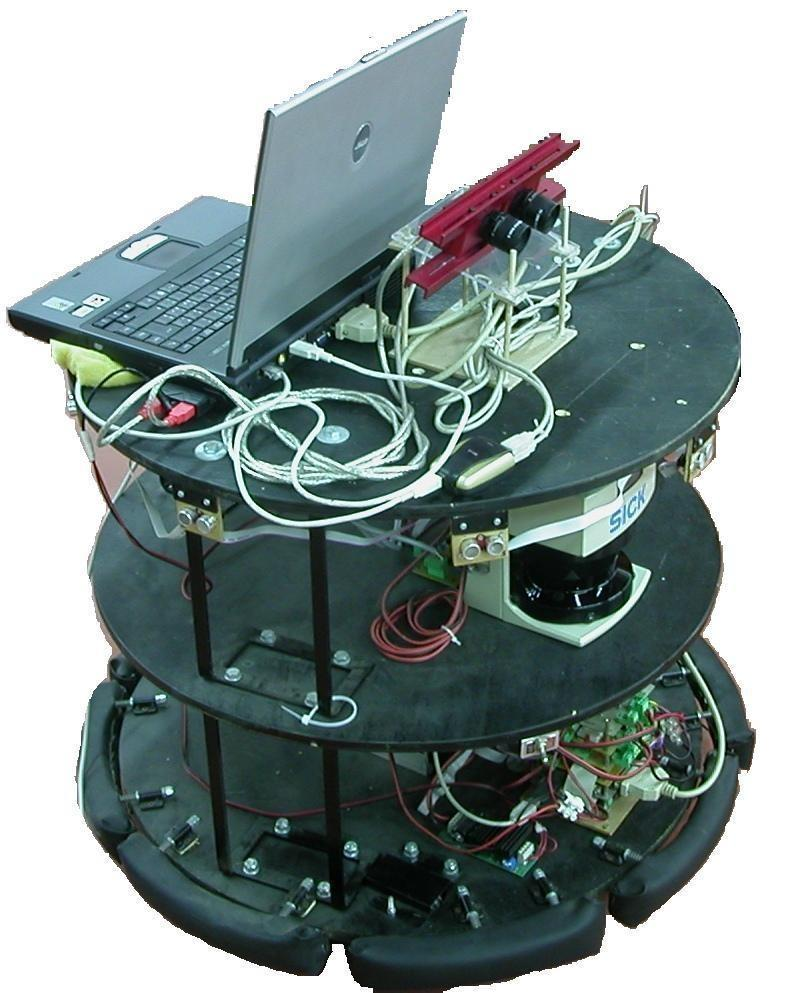
\includegraphics[width=150pt]{img/3morduc.jpg}
    \caption{The 3morduc robotic platform}
    \label{fig:morduc}
  \end{center}
\end{figure}

The telerobot used to develop teleoperation research is
called \textit{3MO.R.D.U.C.}, acronym for `3rd version of
the Mobile Robot DIEES University of Catania'.
3morduc is a mobile-robot, able to move forward, backward
and turn its direction, as directed by the remote operator.
It has been successfully used in several test and experimental
work regarding teleoperation and telepresence.
\\
The robot, actually located at the University of
Catania, is a differential-driven mobile robot, showed
in figure \ref{fig:morduc}.
\\
As every mobile robot, it is equipped with some internal
and external sensors, through which is possible retrieve
information about, respectively, the status of the robot
(e.g. its position) or the data about the environment (e.g.
distance from obstacles).
\\
The moviment is performed by means of two 40W DC engines, model
\textit{Maxon F2260}, connected with the motor shaft by a gear
box (transmission rate 1/19). On the other side the motor shaft
is linked with two rubber wheels, while a third castor wheel can
freely turn to realize the differential-driven model.
\\
The robot is compound by three shelves, each one connected to
the next. On the lower level two lead batteries are situated,
able to erogate 12 Volts at 18 Amperes. The electrical autonomy is
granted for 30-40 minutes.

\begin{figure}
  \begin{center}
    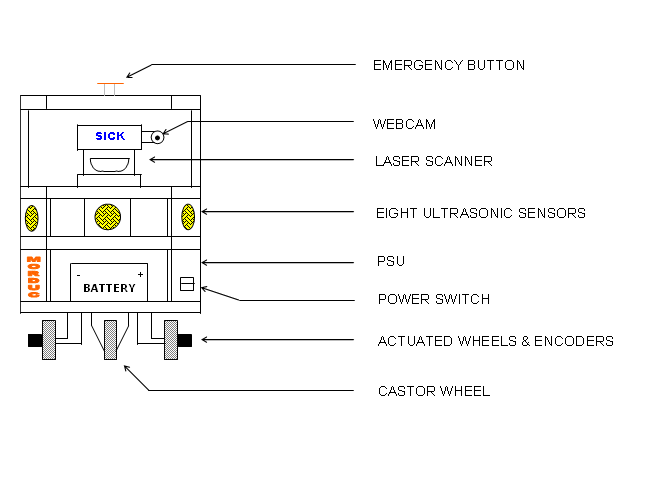
\includegraphics[width=300pt]{img/Morduc_scheme.png}
    \caption{3morduc's schematic figure}
    \label{fig:morduc_scheme}
  \end{center}
\end{figure}

Besides, on the same lower level is located an electronic board
controlling different modules, each one predisposed to manage a
specific task as movements, sensors and communication.
\\
External sensors avaible are:

\begin{itemize}
\item \texttt{belt of bumpers} \\
  A belt of bumpers (in total 16 switches) is dislocated around
  the entire perimeter on the robot base, just over the wheels level.
  The bumpers are simple switches pushed when there is a collision.
  \\
  These sensors recognize clashes between robot and other objects,
  other then reduce damage in case of a collisions.

\item \texttt{incremental encoders} \\
 The two robot motor axes are equipped with incremental encoders, with
 resolution of 500 pulses per turn. These sensors are useful to calculate
 heading and position of the robot by using the kinematic model.  
 \\
 A rotary encoder is shown in figure \ref{fig:encoder}. For more details
 see \ref{sec:3morduc:encoder}.

\item \texttt{belt of sonars} \\
  On the second level are located eight sonar sensors, which measure the
  distance from an obstacle using the flight time of an ultrasonic signal
  produced by means of a vibrating piezoelectric sensor. 
  For more details about sonar sesors see \ref{sec:3morduc:sonar}.

\item \texttt{scanner laser} \\
  In order to detect obstacles on the workspace, the Laser Measurement
  Sensor (LMS) operates by measuring the flight time of a pulsed laser
  light beam that is reflected by obstacle. An internal rotating mirror
  deflects the transmitted pulsed laser beam so that a scan of the
  surrounding area is made. The returned beams is detected by the laser
  receiver. It is possible to configure different angular resolution
  (0.25, 0.5 or 1 degree pace) with different angular scan (100 or 180
  degrees).
  \\
  The time between transmission and reception of the light pulse is directly
  proportional to the distance between the scanner and the object. 
  Further details about LMS can be found in \ref{sec:3morduc:laser}.

\end{itemize}

Internal sensors avaible are:



\begin{comment}

  una stereocamera STH-MDCS2-VAR-C è posta sul top del robot e connessa al PC mediante
●
  l'interfaccia IEEE 1394. Essa è composta da due camere, ciascuna con risoluzione di 1.3
  Megapixel. Il sensore CCD di queste camere ha una buona immunità al rumore e sensibilità.
  Tuttavia è possibile regolare tutti i parametri dell'immagine (exposure gain, frame rate,
  resolution...). Le due camere sono montate su un supporto rigido che permette di regolarne
  la distanza fra loro in un range di 5-20 cm. Le immagini provenienti dalle due camere sono
  sincronizzate ad una frequenza di 8 Khz [5] [6].

On the robot there are also two high quality stereoscopic cameras; each one has a resolution of 1.3 Megapixel; they are equipped with fixed focus lens of 4.0 mm.
The CCD sensors of these cameras have a good noise immunity and sensibility; moreover, it is possible to adjust all the image parameter, e.g.
exposure gain, frame rate, resolution. The cameras are mounted on a rigid support; it permits to simply adjust the camera distance in a range 5-20 cm.






\end{comment}


More images, video and information about 3morduc can
be found in \cite{morduc:features}.


\subsubsection{Encoder section}
\label{sec:3morduc:encoder}

In general, a digital optical encoder is a device that converts motion
into a sequence of digital pulses. The pulses can be converted to relative
or absolute position measurements, by counting a single bit or by decoding
a set of bits.

\begin{figure}
  \begin{center}
    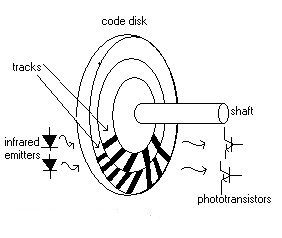
\includegraphics[width=200pt]{img/encoder.jpg}
    \caption{A rotary encoder}
    \label{fig:encoder}
  \end{center}
\end{figure}

In an absolute encoder a unique digital word corresponds to each rotational
position of the shaft, whereas in an incremental encoder (the type mounted
on 3morduc), digital pulses are producted as the shaft rotates,
allowing measurement of the shaft relative position.
\\
The incremental encoder, sometimes also called relative encoder (see figure
\ref{fig:incremental_optical}), is simpler
and cheaper than the absolute encoder. It consists of two tracks and two
sensors whose outputs are called channels A and B.

\begin{figure}
  \begin{center}
    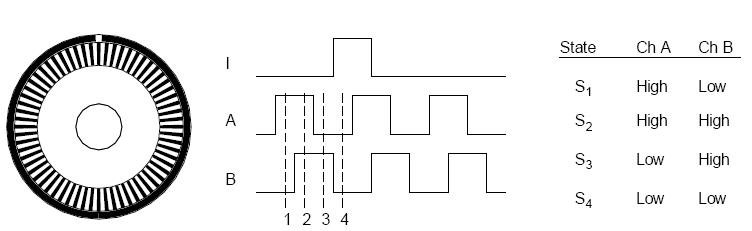
\includegraphics[width=300pt]{img/incremental_optical.jpg}
    \caption{Incremental encoder disk track pattern}
    \label{fig:incremental_optical}
  \end{center}
\end{figure}


As the shaft rotates, pulse trains occur on these channels at a frequency
proportional to the shaft speed and the phase relationship between the
signals yields the direction of rotation. The angular motion can be measured,
by counting the number of pulses and knowing the resolution of the disk.
\\
The A and B channels are used to determine the
direction of rotation by assessing which channels `leads' the other.

\subsubsection{Sonar sensor section}
\label{sec:3morduc:sonar}

Active sonar creates an ultrasonic pulse, often called `ping',
then listens for reflections `echo' (figure \ref{fig:sonar}).

\begin{figure}
  \begin{center}
    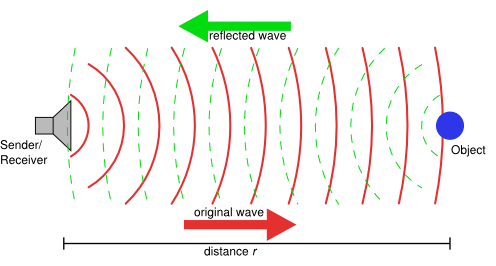
\includegraphics[width=300pt]{img/sonar.png}
    \caption{Sonars in action}
    \label{fig:sonar}
  \end{center}
\end{figure}


The received signal is commonly processed by measuring the time of flight.
This time is depending on the speed of the sound in air, and thus the
temperature, humidity, air pressure, and so on may effect measurements.
\\
The knowledge of time of flight enables the computation of the distance
to the target, which reflected the pulse.
\\
The sonar field of view is a cone and the sensitive area increases proportionately
with the distance. It is necessary to introduce an inhibition time to avoid the false
obstacles due to the ping signal. On the other hand, the inhibition time does
not allow reading distance too short.
\\
The main drawback with the sonar sensor is its wide beam of perception, which
causes the fact that it is impossible from reading returned data to identify
the object position within the beam. Some of the other sonar drawback are specular
reflection; the possibility of a crosstalk when using multiple sensors
or multiple robot.
\\
Nevertheless, the sonar is the sensor most commonly used in robotics, because
widely available, cheap, and easy to controller.


\subsubsection{Laser section}
\label{sec:3morduc:laser}

The Laser sensor is used to measure distance.
\\
The sensor, by a mechanical mechanism with a mirror, sweeps
transmitted and received beams coaxial.
\\
% Figure 2.4: Laser sensor with rotating mirror

The transmitter illuminates a target with a collimated beam
and it received the reflected beam detects the time needed for
round-trip. The distance to an object can be achieved by measuring
the time of flight or the phase shift.
\\
The time of flight is the time between transmission and reception
of the light pulse. This time is directly proportional to the distance
between the scanner and the object.
\\
If you indicate with \textit{L} the distance between the laser and
the obstacle and with \textit{c} the light speed, the proper formula
to retrieve time of fligh is:

\[
t_{flight} = \frac{2L}{c}
\]

so

\[
L = \frac{t_{flight}}{2}c
\]


  
\begin{comment}                          
The quality of time of flight range sensors manly depends on:
         • Uncertainties about the exact time of arrival of the reflected signal
         • Inaccuracies in the time of fight measure
         • Interaction with the target (surface, specular reflections)
         • Variation of propagation speed
         • Speed of mobile robot and target (if not at stand still).
The Phase-Shift measurement produces a range estimation.
We can indicate with:
 f the modulating frequency,
c the light speed,
          c
 λ=          ,
          f
D′ is the distance covered by the emitted light
                                                            θ
                                      D′ = L + 2D = L +         λ
                                                          2 ⋅π
D distance between the beam splitter and the target
                                                    λ
                                                       θ
                                             D=
                                                  4 ⋅π
where θ is the phase difference between the transmitted and the reflected beam.
                          Figure 2.5: Transmitted and Reflected beam
                                                                                        20
                                                                             Chapter 1
Confidence in the range (phase estimate) is inversely proportion to the square of the
received signal amplitude.
In the Figure 2.5 is possible see a typical range image of a 2D laser range sensor with
a rotating mirror. The lengths of the lines through the measurement points indicate
the uncertainties.

\end{comment}
